\subsection{Phase-Specific Capability (PSC)}
%%% RQ6: graded评分揭示二元评分隐藏的差异
%%While 143/150 pairs (95.3\%) would be failures under binary %%evaluation, graded scoring reveals a 23.5-point spread (41.7--65.%%2). Best-of-three scoring adds $\sim$10 points over per-run %%averages, with stronger models showing larger variance (e.g., %%\texttt{glm-5.2}: +14.3), suggesting that succeeding at least once %%is itself a capability dimension.
%%

\begin{figure*}[t]
    \centering
    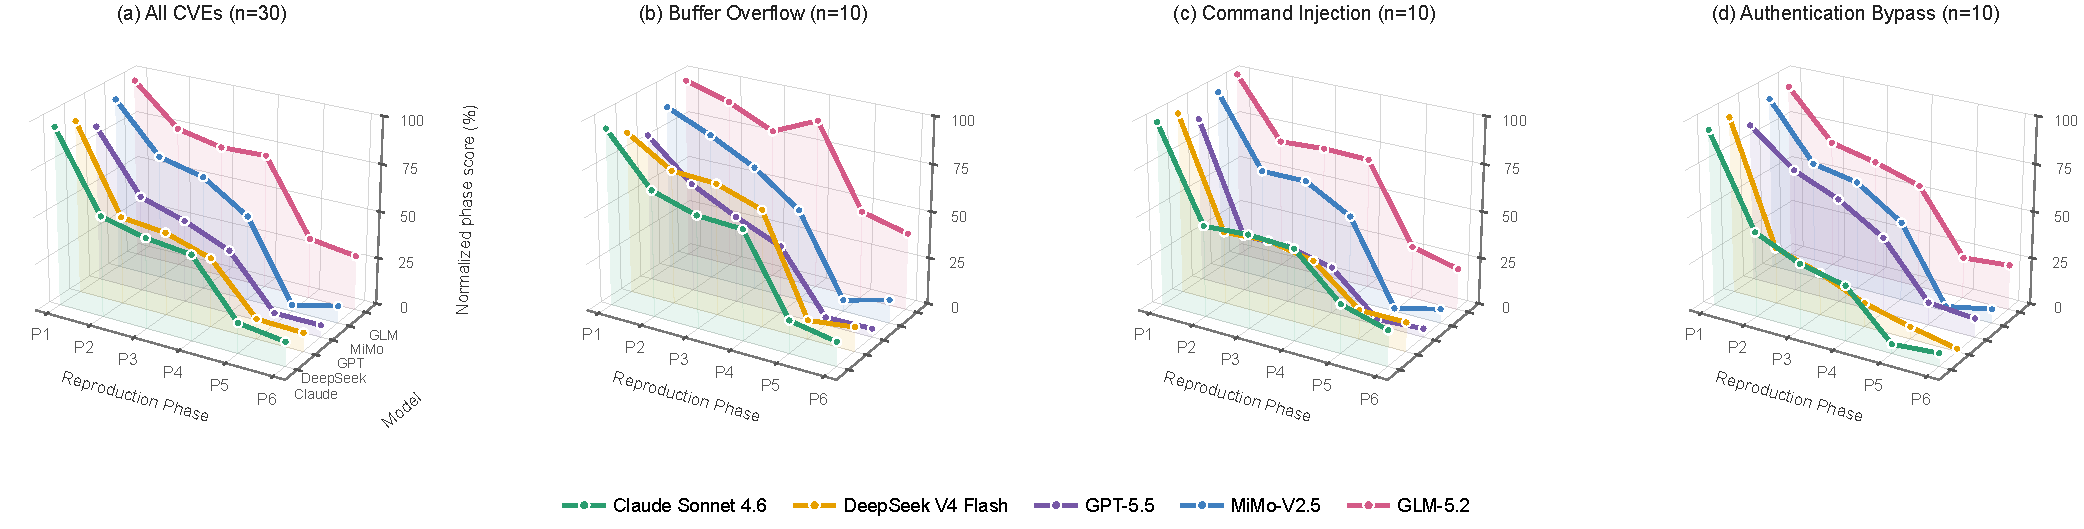
\includegraphics[width=\textwidth]{figures/3d.pdf}
    \caption{Per-phase progress rates across models. P1--P4 show moderate success, but P5 and P6 collapse to near-zero for all models.}
    \label{fig:heatmap}
\end{figure*}

% 异常点分析：19个CVE存在分化，graded评分暴露阶段特定能力
To quantify what capabilities binary metrics conceal, we conduct an anomaly analysis across all 450 runs. We define a \textit{divergence point} where a minority of runs score $\geq$50\% of the phase maximum while a majority score $<$25\%. These two thresholds are chosen to separate genuine capability from attempt-score noise, which caps at $\sim$7\%. For each CVE we select the earliest divergent phase to avoid cascading low scores from unmet prerequisites. We identify 19 scoring results that exhibit such divergence and inspect the \textit{high} and \textit{low} runs' artifacts and trajectories for each. The divergence concentrates at P2 (firmware acquisition, 12/19), P4 (binary identification, 2/19) and P5 (service rehosting, 5/19). We conclude the following three phase-specific capabilities that can improve the success rate of reproduction.

% 三大分化模式：阶段特定能力
\noindent{\textbf{PSC 1: Search Strategy.}} The first divergence point is whether the agent verifies the assumption that firmware is unavailable, written in the plan. High runs test the ``firmware unavailable'' hypothesis by issuing real \texttt{curl} requests to vendor CDNs, regional sites, and community firmware archives. However, low runs just accept the hypothesis without verification and jump to simulation. For example, on CVE-2020-14140, only one of 15 runs actually curls the Xiaomi CDN, discovers the firmware is publicly downloadable, and statically analyzes the extracted Lua controllers; the other 14 runs assume unavailability and produce Python mock servers with zero \texttt{curl} invocations.

\noindent{\textbf{PSC 2: Tooling Knowledge.}} When firmware is encrypted in a vendor-proprietary format, standard \texttt{binwalk} fails and the agent must find out the correct decryption tool. High runs possess domain-specific tooling knowledge to handle encrypted firmware. For example, the \texttt{delink} tool is used for D-Link MH01 encryption, and the correct SHRS decryption key recovered from a sibling model (DIR-3060) is used for DIR-X3260 firmware. However, the low runs assume standard \texttt{binwalk -e} suffices and produce empty extraction. On CVE-2024-6045, only 4/15 runs know the \texttt{delink} tool is required; low runs create empty directories because the default tool cannot process MH01 encryption.

\noindent{\textbf{PSC 3: Rehosting Technique.}} Even with the correct binary extracted, proprietary firmware services fail under QEMU due to missing NVRAM state, kernel ioctl dependencies, and non-standard FastCGI interfaces. High runs employ techniques such as QEMU \texttt{-L} sysroot for library resolution, LD\_PRELOAD NVRAM/nofork stubs, and direct FastCGI socket injection. Low runs hit QEMU failures and switch to C/Python reimplementation. For example, on CVE-2020-13389, the top run (\texttt{glm-5.2}, 19/20) uses QEMU \texttt{-L rootfs} to launch the real Tenda httpd, while a low run using \texttt{chroot} fails on \texttt{br0} ENODEV. On CVE-2023-44418, the top run (\texttt{glm-5.2}, 20/20) identifies \texttt{prog.cgi} as a FastCGI responder and injects protocol frames via a Unix socket; a run with full P1--P4 credit scores only P5=4 by treating it as a standalone web server.

Note that under binary evaluation all 19 divergent CVEs would be uniformly labeled as failures, yet the high runs demonstrate distinct capabilities---hypothesis verification, tool-chain selection, and environment engineering---that are directly transferable to real-world vulnerability analysis but invisible without graded, phase-level scoring.



% \begin{mdframed}[linecolor=black,linewidth=1pt,backgroundcolor=gray!10,roundcorner=3pt,nobreak=true]
% \noindent\textbf{Result-2:} Evidence-grounded scoring reveals distinctions hidden by binary success. Anomaly analysis exposes three phase-specific capabilities that can pass through the bottlenecks.
% \end{mdframed}